\documentclass[10pt,a4paper,notitlepage]{article}
\usepackage[utf8]{inputenc}
\usepackage{amsmath}
\usepackage{amsfonts}
\usepackage{amssymb}
\usepackage{graphicx}
\usepackage[margin=0.5in]{geometry}
\setlength\parindent{0pt}
\title{Crosstalk measurements from PAPER}
\author{Saul A. Kohn$^1$\thanks{saulkohn@sas.upenn.edu}\,\,\,, James E. Aguirre$^1$ \,\,\,\& Chuneeta D. Nunhokee$^{1,2}$\\
$^1$\small{University of Pennsylvania}\\
$^2$\small{Rhodes University} }
\begin{document}
\maketitle

\abstract{Crosstalk is artificial signal created by an interferometer that contaminates the astronomical visibilities it is built to measure. We present extremely compelling evidence that the dominant source of crosstalk for PAPER-64 is reflections between antenna pairs, demonstrating a $1/R^2$ dependence for antenna-separation $R$. Some crosstalk is seen in excess of this trend, and may be due to crosstalk between dipole arms on individual antennae. Under the assumption of identical feeds, we provide the first imaging-based measurements of dipole-arm crosstalk using images from the PAPER-32 imaging configuration. Natural extensions of this work are a full modelling of reflections throughout the array, a more detailed, visibility-based analysis of leakage between dipole arms, and a more complete treatment of polarization calibration.}

\section{Introduction \& Theory}
\label{sec:intro}
XXX Define crosstalk.\\
In this memo, we describe measurements of crosstalk in data from the PAPER-64 EoR observation season and the PAPER-32 polarized-imaging configuration. The former allows us to quantify the effect of total crosstalk on PAPER's standard measurements (which we will show is largely dependent on the antenna configuration), while the latter allows us to probe electronic defects.\\

In this section, we introduce a mathematical model of crosstalk. We outline our measurement techniques in Section~\ref{sec:method}, and present our measurements in Section~\ref{sec:results}. We discuss the implications of our results and conclude in Section~\ref{sec:conc}.


\subsection{Dipole-arm crosstalk}
\label{subsec:theory_dterms}
Crosstalk between dipole arms on a given antenna $m$ can be described by (neglecting noise terms):
\begin{align*}
X'_m = X_m + D^x_mY_m\\
Y'_m = Y_m + D^y_mX_m
\end{align*}
\noindent So an observed $XX$ visibility becomes contaminated by noise-like $XY$ and $YX$ visibilities:
\begin{equation}
X'_mX'_n = X_mX_n + D^x_mY_mX_n + D^x_nX_mY_n  + \mathcal{O}(D^2)
\label{eq:XX_leakage}
\end{equation}
\noindent Which is negligible compared to the $XX$ signal. However, this \textit{polarized leakage} is symmetric, causing $XX$ to leak into $XY$:
\begin{equation}
X'_mY'_n=X_mY_n + D^x_mY_mY_n + D^y_mX_nX_m + \mathcal{O}(D^2)
\end{equation}
\noindent This demonstrates the importance of trying to remove crosstalk when making measurements of polarization -- they will be completely overpowered by the $XX$ and $YY$ terms otherwise.

\subsection{Reflection crosstalk}
\label{subsec:theory_reflection}
We can describe crosstalk from reflections between antenna pair ($m,n$) as:
\begin{equation}
X'_m = X_m + \epsilon^x_{mn}X_n + \epsilon^y_{mn}Y_n;~~~~\epsilon^p_{mn}\propto\frac{1}{|m-n|^2}
\end{equation}
\noindent with a similar definition for $Y_m$; $|m-n|$ represents the physical distance between antennae $m$ and $n$. This means that the observed $XX$ visibility between antennae becomes:
\begin{equation}
X'_mX'_n = X_mX_n + \epsilon^x_{nm}X_mX_m + \epsilon^x_{mn}X_nX_n + \epsilon^y_{nm}X_mY_m + \epsilon^y_{mn}Y_nX_n + \mathcal{O}(\epsilon^2)
\label{eq:XX_reflection}
\end{equation}
\noindent However the $XY$ visibilities are noise-like, so effectively:
\begin{equation}
X'_mX'_n \approx X_mX_n + \epsilon^x_{nm}X_mX_m + \epsilon^x_{mn}X_nX_n 
\end{equation}
\noindent Implying that the observed $XX$ visibilities are contaminated by over-the-air crosstalk from autocorrelations of nearby antennae.

\subsection{Putting it together}
\label{subsec:theory_both}
Using these models, we can represent crosstalk on a given dipole arm as:
\begin{equation}
\begin{pmatrix}
X'_m\\
Y'_m\\
\end{pmatrix}
=
\begin{pmatrix}
1 & D^x_m \\
D^y_m & 1 \\
\end{pmatrix}
\begin{pmatrix}
X_m\\
Y_m\\
\end{pmatrix}
+
\begin{pmatrix}
\epsilon^{xx}_{mn} &\epsilon^{xy}_{mn} \\
\epsilon^{yx}_{mn} &\epsilon^{yy}_{mn} \\
\end{pmatrix}
\begin{pmatrix}
X_n\\
Y_n\\
\end{pmatrix}
\end{equation} 

\noindent We can represent this in a more condensed form as:
\begin{equation}
\vec{m}' = \boldsymbol{D_m}\vec{m} + \boldsymbol{E_{mn}}\vec{n}
\end{equation}
\noindent Such that:
\begin{equation}
\vec{m}'\otimes\vec{n}'
=
\begin{pmatrix}
X_mX_n & X_mY_n \\
Y_mX_n & Y_mY_n\\
\end{pmatrix}
=
(\boldsymbol{D_m}\vec{m} \otimes \boldsymbol{D_n}\vec{n})
+
(\boldsymbol{D_m}\vec{m} \otimes \boldsymbol{E_{nm}}\vec{m})
+
(\boldsymbol{E_{mn}}\vec{n} \otimes \boldsymbol{D_n}\vec{n})
+
(\boldsymbol{E_{mn}}\vec{n} \otimes \boldsymbol{E_{nm}}\vec{m})
\end{equation}

\noindent Neglecting terms $\mathcal{O}(D^2)$, $\mathcal{O}(\epsilon^2)$ and $\mathcal{O}(D\epsilon)$, these outer products reduce as expected:

\begin{equation}
\boldsymbol{D_m}\vec{m} \otimes \boldsymbol{D_n}\vec{n}
\approx
\begin{pmatrix}
X_mX_n + D^x_mY_mX_n + D^x_nX_mY_n    &    X_mY_n + D^x_mY_mY_n + D^y_nX_mX_n \\
Y_mX_n + D^x_nY_mY_n + D^y_mX_mX_n    &    Y_mY_n + D^y_nY_mX_n  + D^y_mX_mY_n \\
\end{pmatrix}
\end{equation}

\begin{equation}
\boldsymbol{D_m}\vec{m} \otimes \boldsymbol{E_{nm}}\vec{m}
\approx
\begin{pmatrix}
\epsilon^{xx}_{nm}X_mX_m + \epsilon^{xy}_{nm}X_mY_m & \epsilon^{yx}_{nm}X_mX_m + \epsilon^{yy}_{nm}X_mY_m  \\
\epsilon^{xx}_{nm}Y_mX_m + \epsilon^{xy}_{nm}Y_mY_m  & \epsilon^{yx}_{nm}Y_mX_m + \epsilon^{yy}_{nm}Y_mY_m   \\
\end{pmatrix}
\end{equation}

\begin{equation}
\boldsymbol{E_{mn}}\vec{n} \otimes \boldsymbol{D_n}\vec{n}
\approx
\begin{pmatrix}
\epsilon^{xx}_{mn}X_nX_n + \epsilon^{xy}_{mn}Y_nX_n    &    \epsilon^{xx}_{mn}X_nY_n + \epsilon^{xy}_{mn}Y_nY_n \\
\epsilon^{yx}_{mn}X_nX_n + \epsilon^{yy}_{mn}Y_nX_n    &    \epsilon^{yx}_{mn}X_nY_n + \epsilon^{yy}_{mn}Y_nY_n \\
\end{pmatrix}
\end{equation}

\noindent and all elements of $\boldsymbol{E_{mn}}\vec{n} \otimes \boldsymbol{E_{nm}}\vec{m}$ are negligible, such that:

\begin{equation}
X'_mX'_n \approx X_mX_n + D^x_mY_mX_n + D^x_nX_mY_n + \epsilon^{xx}_{nm}X_mX_m + \epsilon^{xy}_{nm}X_mY_m + \epsilon^{xx}_{mn}X_nX_n + \epsilon^{xy}_{mn}Y_nX_n 
\end{equation}

\noindent i.e. neglecting crosstalk coupled with the much weaker $XY$ and $YX$ visibilities, we recover the sum of Equations~\ref{eq:XX_reflection} and \ref{eq:XX_leakage}.

\section{Method}
\label{sec:method}

\subsection{Measuring total crosstalk}
\label{subsec:method_xtalk}
We model total crosstalk as if it is constant over time. As shown above, this is not quite true, since the amount of reflection crosstalk is proportional to the autocorrelations, and these in turn are proportional to sky temperature. However, a constant over time is usually a good approximation, especially for the large amount of the season in which the Galaxy is not transiting zenith during observations.\\

Using this constant-over-time model, we proceed with a number of steps to constrain the crosstalk signal based on time-averaged visibilities, extracting the average:
\begin{itemize}
\item  visibility for each baseline, over a 10 minute observation
\item  visibility for each baseline, over a night of observations
\item  visibility for each baseline type over a night of observations
\end{itemize}
\noindent where ``baseline type" refers to a given antenna separation within the PAPER-64 grid. In this case, crosstalk removal is simply a subtraction of the nightly average for each baseline. For analysis of reflection crosstalk we focus on fiducial night JD2456250 from early in the PAPER-64 season, analysing the visibilities between LST=0--8 hours. It has been roughly calibrated to a common Jy scale, allowing for comparisons between baselines. This night has comparable crosstalk levels to other nights in the season, and presents small deviations ($<3\sigma$) from the median sky model at the central frequency of 145\,MHz. The effect of total crosstalk subtraction on a fiducial 30\,m baseline is shown in Figure~\ref{fig:waterfalls}.

\begin{figure}
\centering
\includegraphics[width=0.4\textwidth]{6250_C.png}
\includegraphics[width=0.4\textwidth]{6250_C_d.png}
\includegraphics[width=0.4\textwidth]{6250_Cx.png}
\includegraphics[width=0.4\textwidth]{6250_Cx_d.png}
\caption{\textit{Top}: Waterfall plots of the real part of $YY$ visibilities on a 30\,m baseline in frequency- (left) and delay-space (right). Note the constant-in-time signal on the horizon at positive delay. \textit{Bottom}: the same as above, but after crosstalk subtraction. The bright excess at integration numbers $<$200 is solar. These visibilities have not been CLEANed, leading to noticeable leakage outside of the horizon in delay space.}
\label{fig:waterfalls}
\end{figure}

\subsection{Measuring dipole-arm leakage}
\label{subsec:method_dterms}
The leakage between dipole arms is not configuration dependent. Under the assumption of identical feeds, we can proceed with an imaging-based calibration of the leakage terms using the PAPER-32 polarized imaging configuration following Equations~(4.63) and (4.64) of TMS \cite{TMS}. Assuming Pictor A to be an unpolarized point source, we can make observed $I'$, $Q'$, $U'$ and $V'$ Stokes images of the source at different times, weighting by the beam appropriately.  \\

It follows that the parameters:

\begin{equation}
\delta_{+-} = D^x_m - D^y_m + D^{x*}_n - D^{y*}_n = 2\frac{U'}{I'}
\end{equation}

\begin{equation}
\delta_{-+} = D^x_m + D^y_m - D^{x*}_n - D^{y*}_n = -2\frac{V'}{I'}
\end{equation}

\noindent Which allows us to least-squares solve for the $D$-terms with three observations of the unpolarized source using the formulation:

\begin{equation}
\begin{pmatrix}
\delta_{+-,1} \\
\delta_{-+,1} \\
\delta_{+-,2} \\
\delta_{-+,2} \\
\delta_{+-,3} \\
\delta_{-+,3} \\
\end{pmatrix}
=
\begin{pmatrix}
1 & -1 & 1 & -1 \\
1 & 1 & -1 & -1 \\
1 & -1 & 1 & -1 \\
1 & 1 & -1 & -1 \\
1 & -1 & 1 & -1 \\
1 & 1 & -1 & -1 \\
\end{pmatrix}
\begin{pmatrix}
D^x_{m}\\
D^y_{m}\\
D^{x*}_{n}\\
D^{x*}_{yn}\\
\end{pmatrix}
\label{eq:Dterms3times}
\end{equation}

\subsection{Measuring individual reflections}
\label{subsec:method_reflections}

Measuring reflections independent of total crosstalk is a difficult endeavour, outside the scope of this memo. Since the $\epsilon^{pq}_{ij}$ values are coupled to autocorrelations throughout the array, one needs to model each dipole `broadcasting' a fraction of its autocorrelation to every other antenna. If we consider the case of no D-term leakage, as written in Equation~\ref{eq:XX_reflection}, we see that even in the limit of autocorrelations being unaffected by crosstalk (i.e. $X'_mX'_m=X_mX_m$) there are still 3 unknown parameters per visibility: the `true' visibility $X_mX_n$, $\epsilon^{xx}_{mn}$ and $\epsilon^{xy}_{mn}$. This crosstalk will technically vary on the timescale of a single autocorrelation, so it is difficult to argue for the least-squares technique used to solve for the D-terms, which assumes couplings that are constant in time.

\section{Results}
\label{sec:results}

\subsection{Total crosstalk}
In Figure~\ref{fig:xtalk-per-file}, we show the average visibility on a fiducial 30\,m baseline for each 10 minute integration (left) and the total average (right) over JD2456250. Close to the start of the observation season, the Galaxy is not present in this data. Sunset can be seen, with much larger average visibilities at the start of the night (top; note that the sun is technically below the horizon at this time). The dip at 137\,MHz is the always-flagged ORBCOMM satellite band. The flat lines on both ends of the spectrum are the always-flagged band edges. Note that the total crosstalk in any given integration appears to be roughly constant, but that it does change in profile throughout the night. In the night-average profile, it is interesting to note that the lowest points in the spectrum ($\sim150-175$\,MHz) roughly corresponds to the quietest part of the band in terms of RFI (Kohn et al. HERA memo in prep.). This data has already been RFI-flagged twice, once in high and once in low spectral resolution. \\

\begin{figure}
\centering
\includegraphics[width=0.4\textwidth]{6250_yy_xtalk_per_file.png}
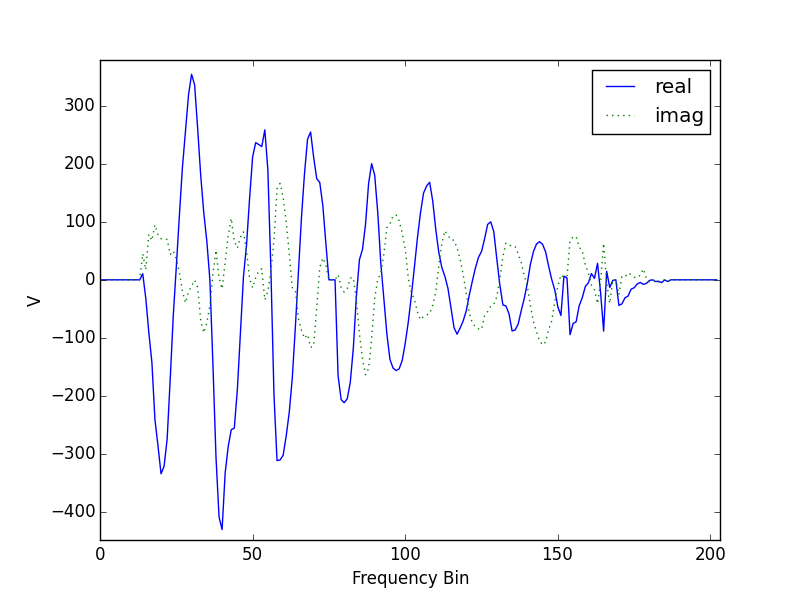
\includegraphics[width=0.4\textwidth]{mean_xtalk_all_1unit_BLs_6250.png}
\caption{\textit{Left}: The average $YY$ (absolute-value) visibility for a single 30\,m baseline of each 10 minute file over the night, plus a constant offset for display purposes. The average of the first file is at the top, and file time progresses downwards. \textit{Right}: The time-averaged visibility for that baseline over the night.}
\label{fig:xtalk-per-file}
\end{figure}

\subsection{Reflections}
Consider a plane wave incident on antenna $m$, which reflects onto antenna $n$. Such a reflected signal would have a delay corresponding to the distance between the antennae. We can investigate the presence of such reflections by delay-transforming the average visibilities of different baseline-types and looking for resonances at the corresponding delays. An example of this method is shown in Figure~\ref{fig:xtalk-for-BL1}, which shows the night-averaged visibilities on all of the 30\,m baselines in the array (left) and the median of those signals (right). In both plots, there is a clear resonance exactly at the delay corresponding to the 30\,m baseline length in both directions, suggesting that reflections are dominating the crosstalk signal.\\

\begin{figure}
\centering
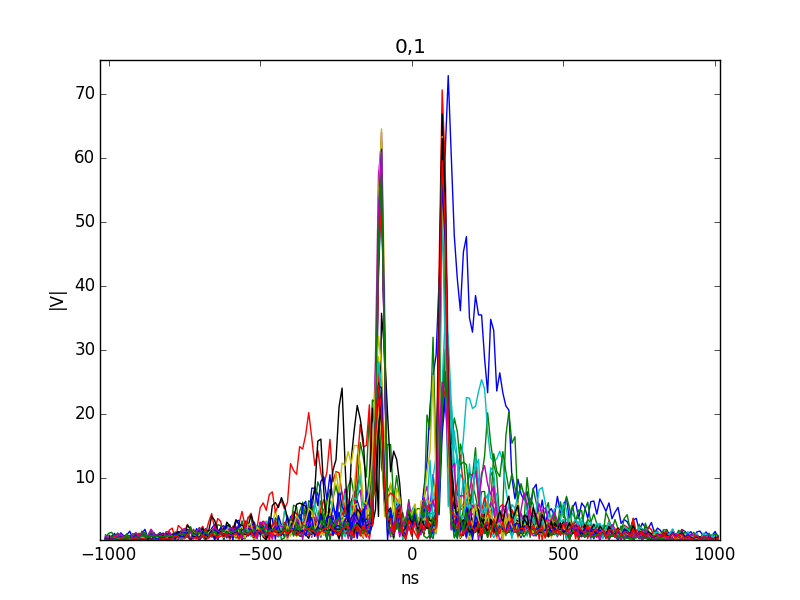
\includegraphics[width=0.4\textwidth]{6250_yy_xtalk_that_night_BLtype1_d.png}
\includegraphics[width=0.4\textwidth]{6250_yy_xtalk_that_night_BLtype1_median_d.png}
\caption{\textit{Left}: The delay transform of the average signal for the night for all 30\,m baselines in the array (`bad antennae' identified by OMNICAL have been removed). \textit{Right}: The average of these signals. The dotted lines show the light-travel-time between increasing grid separations (1, 2, 3 and 4-unit separations).}
\label{fig:xtalk-for-BL1}
\end{figure}

We make a further test of the hypothesis that the dominant source of crosstalk is reflections by measuring the average crosstalk on each baseline type (30, 60, 90 and 120\,m baselines). These are shown in Figure~\ref{fig:the-money-plot}; indeed, we see the maximum signal in delay-space (which always lines-up with baseline separation delays) decrease by approximately a factor of 4 for each increase in spacing, i.e. a $1/R^2$ dependence.\\

\begin{figure}
\centering
\includegraphics[width=0.4\textwidth]{xx_1unit_xtalk_d.png}
\includegraphics[width=0.4\textwidth]{xx_2unit_xtalk_d.png}
\includegraphics[width=0.4\textwidth]{xx_3unit_xtalk_d.png}
\includegraphics[width=0.4\textwidth]{xx_4unit_xtalk_d.png}
\includegraphics[width=0.4\textwidth]{max.png}
\caption{The average signal over the night in delay-space, averaged for baseline types of 30, 60, 90 and 120\,m separations. Also shown is the relationship between the maximum value of the delay spectrum in comparison to a $1/R^2$ falloff, which it loosely follows.}
\label{fig:the-money-plot}
\end{figure}

It is important to understand the magnitude of crosstalk compared to typical visibilities. This is a little difficult to communicate effectively, since we have measured crosstalk under the definition of a time-average over the visibilities. However, if define a parameter $\xi_V$: 

\begin{equation}
\xi_V=\frac{1}{T}\sum_t\frac{V(\nu)}{\sqrt{\sum_\nu|V(\nu)|^2}}
\end{equation}

That is, time- and baseline-averaged visibilities weighted by their RMS over frequency at each integration, should give a measure of how much crosstalk is present at each delay. This statistic is shown in Figure~\ref{fig:xi_V}, and several interesting features are apparent. The 30\,m baselines have excess power in `wings', loosely corresponding to the 60\,m and 90\,m separations. The longer baselines may have these wings also, but at the level of noise. The noise inside the horizon on the 30\,m baselines is comparable to the total crosstalk on the 120\, baselines.
Note that this all occurs at levels $\sim0.1-1.5\%$ of the total (foreground) signal. This means that once we have averaged backgrounds to levels 1\% of the original visibilities, reflection crosstalk will dominate and prevent further averaging-down. \\
XXX NEED THE CONVERSION FROM NANOSECONDS TO K-SPACE TO SEE IF THIS MIGHT CONTRIBUTE TO DAMO-BUMPS\\
%well this looks scary

\begin{figure}
\centering
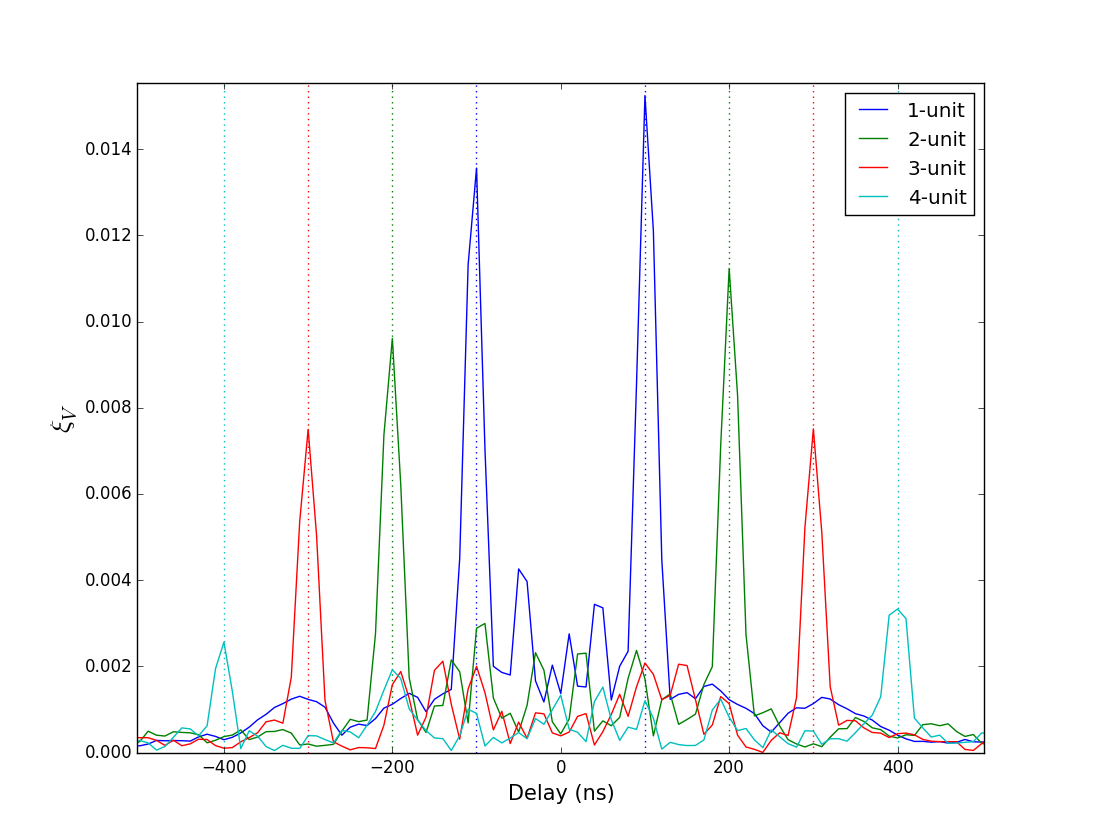
\includegraphics[scale=0.5]{xi_V-zoom.png}
\caption{The value of $\xi_V$ is a measure of how much total crosstalk is present in visibilities on average.}
\label{fig:xi_V}
\end{figure}

\subsection{D-terms}

Using the PAPER-32 polarized imaging array data from JD2455819, we used crosstalk-subtracted $X'X'$, $X'Y'$, $Y'X'$ and $Y'Y'$ visibilities, ported into CASA, to make images, averaging over all frequencies to boost signal-to-noise. Stokes images were formed by combining images according to:

\begin{equation}
\begin{pmatrix}
I' \\
Q' \\
U' \\
V' \\
\end{pmatrix}
=\frac{1}{2}
\begin{pmatrix}
1 & 0 & 0 & 1 \\
-1& 0 & 0 & 1 \\
0 & 1 & 1 & 0 \\
0 & i & -i & 0 \\
\end{pmatrix}
\begin{pmatrix}
X'X' \\
X'Y' \\
Y'X' \\
Y'Y' \\
\end{pmatrix}
\end{equation}

Within this night, Pictor A transited close to zenith, and we used three integrations closets to transit (minimizing wide-field effects). At each integration, the flux of Pictor A was measured in $I'$, $U'$ and $V'$ to form the $\delta$ parameters. We used these to calculate the D-terms as described in Equation~\ref{eq:Dterms3times}.\\  

XXX The results of this experiment were:\\
\begin{align*}
XXX\\
XXX\\
XXX\\
XXX
\end{align*}

Using these values, we could correct for D-term leakage in the image plane:
\begin{equation}
U = U' - \delta_{+-}I'
\end{equation}
\begin{equation}
V = V' - \delta_{-+}I'
\end{equation}


XXX IMAGES, SOME INTERPRETATION 

\section{Discussion \& Conclusions}
\label{sec:conc}

\subsection{Why we care}
\begin{itemize}
\item Crosstalk is non-astrophysical, but redundant calibration techniques such as OMNICAL \cite{Zheng} are `sky-agnostic' and will attempt to calibrate contaminated data, leading to incorrect antenna gains and, for example, therefore risking greater $Q' \rightarrow I'$ leakage.
\item Most of the crosstalk power lies outside of the horizon, especially on the shortest baselines, limiting our ability to probe the EoR window in any analysis and especially in foreground-avoidance methods such as DDR-filtering \cite{Parsons}.
\item Inaccurate crosstalk subtraction leaves artefacts in images (stripes of constant declination) which will be detrimental for imaging-based calibration such as FHD \cite{Sullivan}.
\item Without any accounting for crosstalk, the $XY$ and $YX$ visibilities are completely overpowered by crosstalk coupled to $XX$ and $YY$ correlations, limiting our ability to constrain astrophysical polarization as a separate contaminant of the EoR window.
\end{itemize}

\subsection{Implications for HERA}

Using the formalism laid-out at the start of this memo, we hope to move forward with a common language for the collaboration to talk about crosstalk. Additions are of course welcome. We have also presented a technique for measuring crosstalk (which is being implemented for the polarized PAPER-64 power spectrum analyses and all of the PAPER-128 analyses), and shown the expected delay spectra in the presence of strong reflections. The simple method presented in this memo for calculating D-term leakage is a strong motivator for regularly imaging in four polarizations.

HERA-19, now under construction in South Africa, and HERA-GB, 3 dish prototypes in Green Bank, WV, are based on design choices drawing from lessons learned from PAPER, MWA and OMNISCOPE. Different crosstalk mitigation strategies will be tested -- primarily with HERA-GB -- such as erecting `fences' around the rim of each HERA dish.
Given the points above, particular care and attention should be given to the characteristics of average visibilities in delay-space with and without crosstalk mitigation.


\bibliographystyle{plain}
\bibliography{xtalkmemoBib}

\end{document}